\documentclass{standalone}
\usepackage{amsmath}
\usepackage{graphicx}
\usepackage{subfig}
\usepackage{booktabs}
\usepackage{tikz}
\usetikzlibrary{arrows.meta}
\usepackage{comment}

\begin{document}

\begin{tabular}{lcccc}
% Header row
& \multicolumn{2}{c}{\textbf{\textsf{System 1}}} & \multicolumn{2}{c}{\textbf{\textsf{System 2}}} \\
% Midrule under headers
\cmidrule(lr){2-3} \cmidrule(lr){4-5}
% Sub-header row
& \textsf{Symbolic} & \textsf{Graphical} & \textsf{Graphical} & \textsf{Symbolic} \\
% Midrule under sub-headers
\cmidrule(lr){2-2} \cmidrule(lr){3-3} \cmidrule(lr){4-4} \cmidrule(lr){5-5}
% Row with time series
\rotatebox[origin=c]{90}{\textsf{Time series}}
&
\begin{minipage}{0.49\textwidth}
% {} needed around align in tabular. See: https://tex.stackexchange.com/questions/121407/align-inside-of-tabular
{\begin{align*}
	x &= \left( x_1, x_2, \ldots, x_n \right) \\
	y &= \left( y_1, y_2, \ldots, y_n \right) \\
	z &= \left( z_1, z_2, \ldots, z_n \right)	
\end{align*}}
\end{minipage}
&
\begin{minipage}{0.49\textwidth}
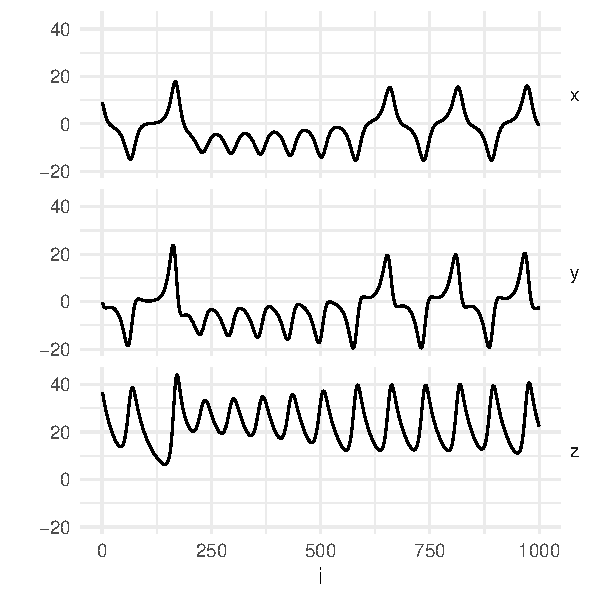
\includegraphics[width=\textwidth]{ts_1.pdf}
\end{minipage}
&
\begin{minipage}{0.49\textwidth}
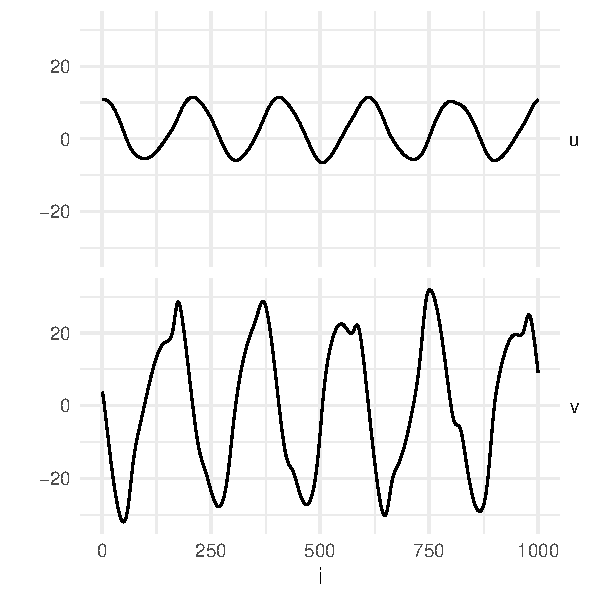
\includegraphics[width=\textwidth]{ts_2.pdf}
\end{minipage}
&
\begin{minipage}{0.49\textwidth}
{\begin{align*}
	u &= \left( u_1, u_2, \ldots, u_n \right) \\
	v &= \left( v_1, v_2, \ldots, v_n \right)	
\end{align*}}
\end{minipage}
\\
% Row with arrows pointing down
\rotatebox[origin=c]{90}{\textsf{Embedding}}
&
\begin{minipage}{0.49\textwidth}
\centering
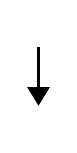
\begin{tikzpicture}
	\node[name=t] at (0, 1) {};
	\node[name=b] at (0, 0) {};
	\draw[-Triangle, line width=0.5mm] (t) to (b);
\end{tikzpicture}
\end{minipage}
&
\begin{minipage}{0.49\textwidth}
\centering
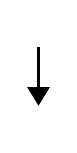
\begin{tikzpicture}
	\node[name=t] at (0, 1) {};
	\node[name=b] at (0, 0) {};
	\draw[-Triangle, line width=0.5mm] (t) to (b);
\end{tikzpicture}
\end{minipage}
&
\begin{minipage}{0.49\textwidth}
\centering
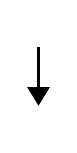
\begin{tikzpicture}
	\node[name=t] at (0, 1) {};
	\node[name=b] at (0, 0) {};
	\draw[-Triangle, line width=0.5mm] (t) to (b);
\end{tikzpicture}
\end{minipage}
&
\begin{minipage}{0.49\textwidth}
\centering
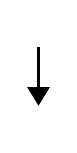
\begin{tikzpicture}
	\node[name=t] at (0, 1) {};
	\node[name=b] at (0, 0) {};
	\draw[-Triangle, line width=0.5mm] (t) to (b);
\end{tikzpicture}
\end{minipage}
\\
% Row with phase space plots
\rotatebox[origin=c]{90}{\textsf{Phase space}}
&
\begin{minipage}{0.49\textwidth}
$$
	\mathbf{X} =
	\begin{pmatrix}
		x_1 & y_1 & z_1 \\
		x_2 & y_2 & z_2 \\
		\vdots & \vdots & \vdots \\
		x_n & y_n & z_n
	\end{pmatrix}
$$
\end{minipage}
&
\begin{minipage}{0.49\textwidth}
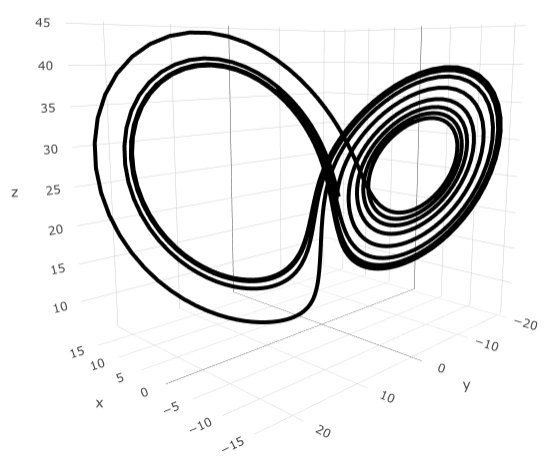
\includegraphics[width=\textwidth]{ps_1.png}
\end{minipage}
&
\begin{minipage}{0.49\textwidth}
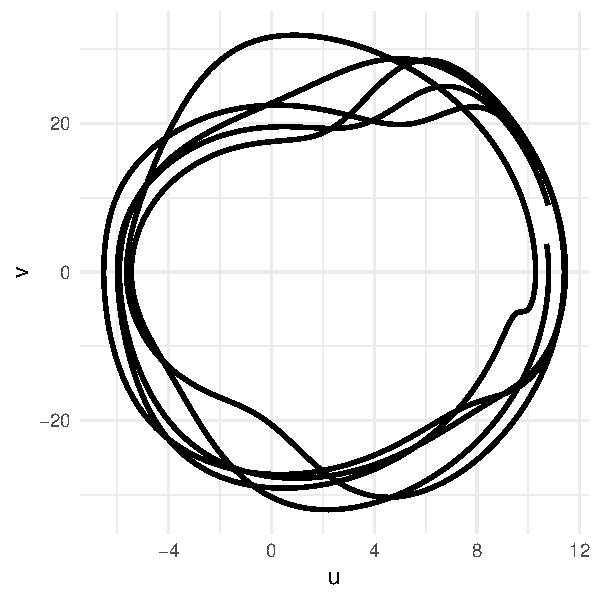
\includegraphics[width=\textwidth]{ps_2.pdf}
\end{minipage}
&
\begin{minipage}{0.49\textwidth}
$$
	\mathbf{Y} =
	\begin{pmatrix}
		u_1 & v_1 \\
		u_2 & v_2 \\
		\vdots & \vdots \\
		u_n & v_n
	\end{pmatrix}
$$
\end{minipage}
\\
% Row with arrows pointing down
\rotatebox[origin=c]{90}{\textsf{MdRQA}}
&
\begin{minipage}{0.49\textwidth}
\centering
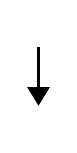
\begin{tikzpicture}
	\node[name=t] at (0, 1) {};
	\node[name=b] at (0, 0) {};
	\draw[-Triangle, line width=0.5mm] (t) to (b);
\end{tikzpicture}
\end{minipage}
&
\begin{minipage}{0.49\textwidth}
\centering
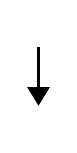
\begin{tikzpicture}
	\node[name=t] at (0, 1) {};
	\node[name=b] at (0, 0) {};
	\draw[-Triangle, line width=0.5mm] (t) to (b);
\end{tikzpicture}
\end{minipage}
&
\begin{minipage}{0.49\textwidth}
\centering
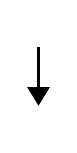
\begin{tikzpicture}
	\node[name=t] at (0, 1) {};
	\node[name=b] at (0, 0) {};
	\draw[-Triangle, line width=0.5mm] (t) to (b);
\end{tikzpicture}
\end{minipage}
&
\begin{minipage}{0.49\textwidth}
\centering
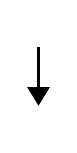
\begin{tikzpicture}
	\node[name=t] at (0, 1) {};
	\node[name=b] at (0, 0) {};
	\draw[-Triangle, line width=0.5mm] (t) to (b);
\end{tikzpicture}
\end{minipage}
\\
% Row with Recourrence plots
\rotatebox[origin=c]{90}{\textsf{Recurrence plots}}
&
\begin{minipage}{0.49\textwidth}
\begin{equation*}
	\mathbf{X}_i = (x_i, y_i, z_i)
\end{equation*}\\[2ex]
\begin{equation*}
    R_{X,ij} = 
    \begin{cases} 
      1 & \quad \text{if}\quad \|\mathbf{X}_i - \mathbf{X}_j\| \leq \varepsilon_X \\
      0 & \quad \text{if}\quad \| \mathbf{X}_i - \mathbf{X}_j \| > \varepsilon_X
   \end{cases}
\end{equation*}
\end{minipage}
&
\begin{minipage}{0.49\textwidth}
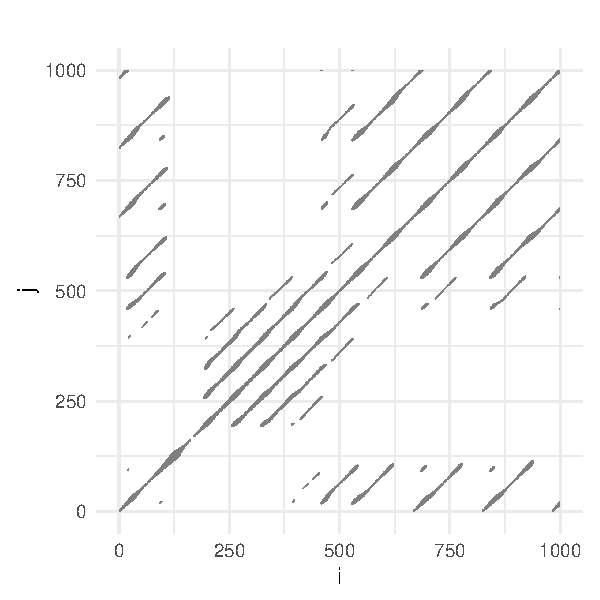
\includegraphics[width=\textwidth]{rp_1.pdf}
\end{minipage}
& 
\begin{minipage}{0.49\textwidth}
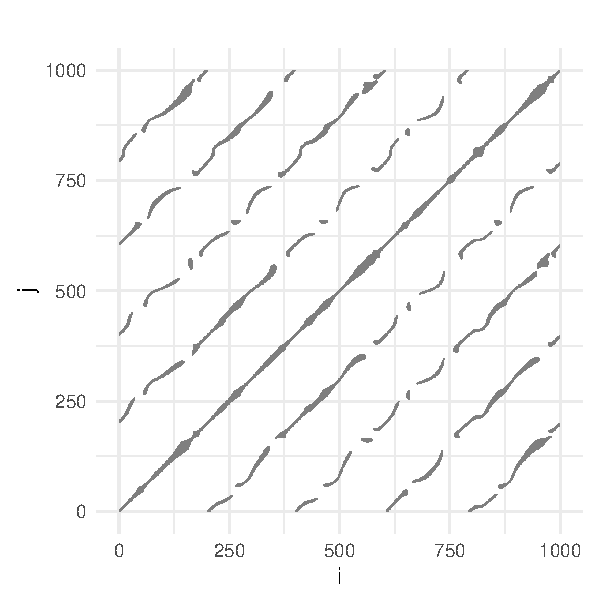
\includegraphics[width=\textwidth]{rp_2.pdf}
\end{minipage}
&
\begin{minipage}{0.49\textwidth}
\begin{equation*}
	\mathbf{Y}_i = (u_i, v_i)
\end{equation*}\\[2ex]
\begin{equation*}
    R_{Y,ij} = 
    \begin{cases} 
      1 & \quad \text{if}\quad \|\mathbf{Y}_i - \mathbf{Y}_j\| \leq \varepsilon_Y \\
      0 & \quad \text{if}\quad \| \mathbf{Y}_i - \mathbf{Y}_j \| > \varepsilon_Y
   \end{cases}
\end{equation*}
\end{minipage}
\\
% New header row
& & \multicolumn{2}{c}{\textbf{\textsf{Combined system}}} &  \\
% Midrule under headers
\cmidrule(lr){3-4}
% Sub-header row
& & \textsf{Symbolic} & \textsf{Graphical} &   \\
% Midrule under sub-headers
\cmidrule(lr){3-3}  \cmidrule(lr){4-4}
% Row with JRP and arrows from above
\rotatebox[origin=c]{90}{\textsf{Joint recurrence plot}}
&
\multicolumn{2}{r}{
	\begin{minipage}[t]{0.1\textwidth}
		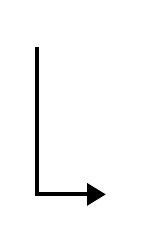
\begin{tikzpicture}
			\node[name=t] at (0, 2) {};
			\node[name=b] at (1, 0) {};
			\draw[-Triangle, line width=0.5mm] (t) |- (b);
		\end{tikzpicture}
		\end{minipage}
		\begin{minipage}{0.49\textwidth}
		\begin{equation*}
			\mathbf{J} = \mathbf{R}_X \circ \mathbf{R}_Y
		\end{equation*}\\[2ex]
		\begin{equation*}
			J_{ij} = 
    		\begin{cases} 
      		1 & \quad \text{if}\quad 
			\begin{array}{l}
				\|\mathbf{X}_i - \mathbf{X}_j\| \leq \varepsilon_X \\
			 	\|\mathbf{Y}_i - \mathbf{Y}_j\| \leq \varepsilon_Y \\
			\end{array}
			\\
      		0 & \quad \text{otherwise}
   			\end{cases}
		\end{equation*}
		\end{minipage}
}
&
\multicolumn{2}{l}{
	\begin{minipage}{0.49\textwidth}
		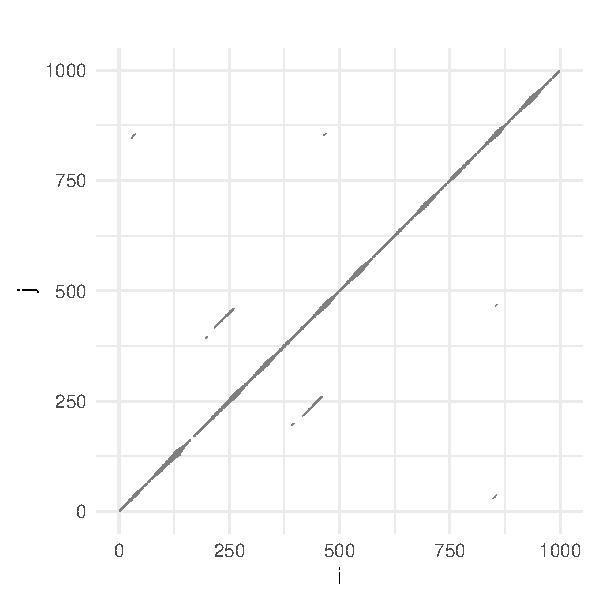
\includegraphics[width=\textwidth]{jrp.pdf}
	\end{minipage}
	\begin{minipage}[t]{0.1\textwidth}
		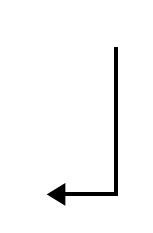
\begin{tikzpicture}
			\node[name=t] at (0, 2) {};
			\node[name=b] at (-1, 0) {};
			\draw[-Triangle, line width=0.5mm] (t) |- (b);
		\end{tikzpicture}
	\end{minipage}
}
\begin{comment}
\end{comment}
\end{tabular}

\end{document}


